\documentclass[a4paper,11pt]{article}
\usepackage{latexsym}
\usepackage[italian]{babel}
\usepackage[utf8]{inputenc}  
\usepackage{pdfsync}
\usepackage{moreverb}
\usepackage{listings}
\usepackage{graphicx}
\author{Alessio Caiazza, Cosimo Cecchi}
\title{CaptureMJPEG: a MotionJPEG library for Procesing}
\frenchspacing
\begin{document}
\maketitle

\newcommand{\reffigura}[1]{
  Figura \ref{#1}
}

\begin{abstract}
CaptureMJPEG è una libreria per
Processing\footnote{http://processing.org} che consente di gestire uno
stream motion-jpeg come input video.\\
La libreria è in grado di acquisire lo stream tramite i protocolli
\mbox{HTTP/HTTPS} e dispone di alcune classi di aiuto per la generazione di
URL per le videocamere di rete AXIS e Sony.  
\end{abstract}
\tableofcontents


\section{Introduzione}
\label{sec:introduzione}
%Cosa è stato fatto, come e con quali obiettivi
%Presentazione del progetto e del sito


\section{Manuale}
\label{sec:manuale}
Guida all'installazione ed utilizzo di CaptureMJPEG
\subsection{Installazione}
\label{sec:installazione}
%scopiazzare dal sito e tradurre in italiano
Per prima cosa scaricare l'ultima versione di CaptureMJPG dal sito
ufficiale http://capturemjpeg.lilik.it .\\
Una volta ottenuto l'archivio decomprimerlo all'interno della
sottocartella \texttt{contributed} del proprio sketchbook, su Linux
solitamente è \texttt{$\sim$/sketchbook}, su Mac OS X e Windows
è la cartella \texttt{Processing} all'interno dei propri documenti.\\
Qualora la sottocartella \texttt{contributed} non esistesse è
necessario crearla.\\
A questo punto riavviare Processing. 
\subsection{Guida all'utilizzo}
\label{sec:guida}
%inserire un po' di esempi e spiegare le funzioni utilizzabili



\section{Analisi}
\label{sec:analisi}

\subsection{Comparazione dell'algoritmo blur fra CaptureMJPEG e Capture}
\label{sec:comparazione}

%Studio della libreria eseguito con il codice di prova
L'analisi è stata svolta applicando un filtro \texttt{blur} allo
stream ottenuto con CaptureMJPEG e con la videocamera locale
utilizzando la libreria Capture\footnote{la libreria Capture è fornita
  in bundle con Processing.}.\\
I sorgenti utilizzati sono quelli in \reffigura{fig:micc_blur} per
CaptureMJPEG e in \reffigura{fig:capture_blur} per Capture.
Sono stati misurati l'utilizzo di memoria e di CPU al variare delle
dimensioni del filmato e del framerate richiesto allo sketch.\\
\begin{figure}
  \centering
\lstinputlisting[language=Java,numbers=left,frame=shadowbox]{sources/micc_blur.pde}  
  \caption{Sorgente di test CaptureMJPEG}
  \label{fig:micc_blur}
\end{figure}
\begin{figure}
  \centering
  \lstinputlisting[language=Java,numbers=left,frame=shadowbox]{sources/capture_blur.pde}
  \caption{Sorgente di test Capture}
  \label{fig:capture_blur}
\end{figure} 
L'analisi ha riportato un utilizzo di memoria minore per la libreria
CaptureMJPEG, 30MB contro 40MB per il filmato a risoluzione 320x240 e
50MB contro 60MB per il filmato a risoluzione 640x480.\\

\begin{figure}
  \centering
  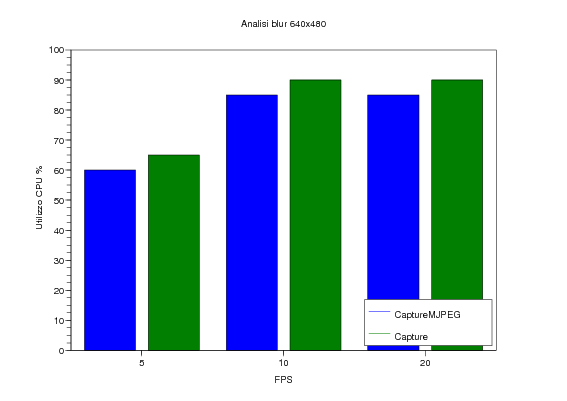
\includegraphics[scale=0.9]{scilab/isto_blur_640.png}
  \caption{Analisi algoritmo blur 640x480}
  \label{fig:blur_640}
\end{figure}
\begin{figure}
  \centering
  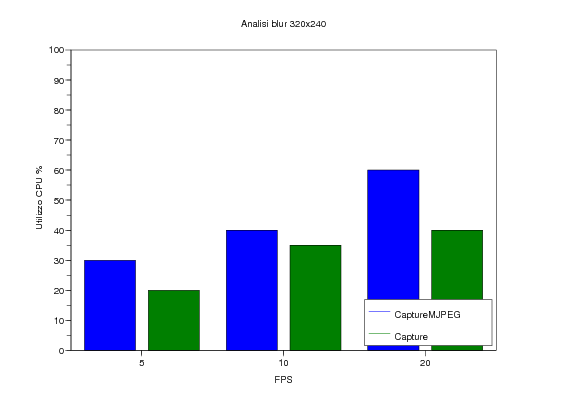
\includegraphics[scale=0.9]{scilab/isto_blur_320.png}
  \caption{Analisi algoritmo blur 320x240}
  \label{fig:blur_320}
\end{figure}

L'utilizzo di CPU è riportato in \reffigura{fig:blur_640} e in
\reffigura{fig:blur_320}.
L'algoritmo applicato allo stream di risoluzione 320x240 mostra un
utilizzo di CPU più pesante da parte di CaptureMJPEG in media del
11.7\% mentre con lo stream a risoluzione 640x480 l'utilizzo è più
pesante da parte della libreria Capture, con un distacco fisso del
5\%.\\
Si deve considerare inoltre il fatto che CaptureMJPEG utilizza
connessioni HTTP remote mentre Capture utilizza il bus USB ad alta
velocità del sistema locale.\\

I test sono stati eseguiti su un iMac con la seguente configurazione:
\begin{tabbing}
  \textbf{sistema operativo} \= Mac OS X 10.4.11 \kill

  \textbf{processore} \>Intel Core Duo 2GHz (32 bit, dual core)\\
  \textbf{memoria RAM} \> 1GB a 667MHz \\
  \textbf{sistema operativo} \> Mac OS X 10.4.11 \\
  \textbf{processing} \> 0135 beta \\
\end{tabbing}

\subsection{Impressioni qualitative}
\label{sec:impressioni}

%andrebbe scritto in italiano! :P
Le modalità callback si presta bene per la realizzazione di sketch con
funzionalità di monitoring, mentre se si richiede di processare i
frame acquisiti si consiglia l'utilizzo della modalità senza callback
se si preferisce diminuire il delay perdendo frame di immagine, se
è più importante processare tutti i frame, anche acquisendo un
notevole ritardo rispetto alla scena ripresa, allora utilizzare la
modalità con callback.

\section{Sviluppo}
\label{sec:sviluppo}
Come continuare lo sviluppo
\subsection{Ottenere i sorgenti}
\label{sec:sorgenti}
Prima di scaricare i sorgenti è necessario installare
Mercurial\footnote{Mercurial può essere scaricato dal sito
 http://www.selenic.com/mercurial/}, 
per la gestione dei sorgenti ed Ant\footnote{Ant può essere scaricato
dal sito http://ant.apache.org}, 
per la gestione della compilazione.

Per ottenere i sorgenti eseguire la clonazione del repository
mercurial disponibile all'indirizzo
\texttt{http://dev.abisso.org/capturemjpeg} 
dopodiché creare una copia del file \texttt{user\_pref.xml.template}
con nome \texttt{user\_pref.xml}.

Il file contiene la configurazione di ant per il progetto, tutti i
valori di default vanno bene ad eccezione della ``property''
\texttt{processing-core} che deve essere corretta con la path completa
al file \texttt{core.jar} incluso nella propria installazione di Processing.
\begin{verbatim}
<property name="processing-core" 
    value="C:\Programmi\processing-0135-expert\lib\core.jar" />
\end{verbatim}

A questo punto è necessario eseguire il dowload delle librerie incluse
in CaptureMJPEG eseguendo il comando:
\begin{verbatim}
   ant download_deps
\end{verbatim}

Quindi è possibile generare l'intera cartella di installazione con
il comando:
\begin{verbatim}
   ant deploy 
\end{verbatim}
\begin{figure}
  \centering
\begin{boxedverbatim}

 hg clone http://dev.abisso.org/capturemjpeg capturemjpeg   
 cd capturemjpeg
 cp user_pref.xml.template user_pref.xml

\end{boxedverbatim}  
  \caption{Come ottenere i sorgenti da terminale}
  \label{fig:clone}
\end{figure}

\subsection{Classi utilizzate}
\label{sec:classi}
Forniamo ora una descrizione sommaria delle classi sviluppate per la
libreria, per una trattazione più approfondita si rimanda alla
documentazione JavaDoc disponibile online all'indirizzo 
http://capturemjpeg.lilik.it/doc/

%inserire il diagramma delle classi UML e aggiungere qualche commento




\end{document}
